\documentclass[11pt]{article}
\usepackage[top=0.9in,bottom=1in,left=0.75in,right=0.75in]{geometry}
\usepackage{amsmath, amssymb}
\usepackage{enumitem}
\usepackage{graphicx}
\usepackage{xcolor}
\usepackage{listings}
\usepackage{titling}
\setlength{\abovedisplayskip}{4pt}
\setlength{\belowdisplayskip}{4pt}
\setlength{\abovedisplayshortskip}{2pt}
\setlength{\belowdisplayshortskip}{2pt}
\setlength{\jot}{2pt}
\setlist{nosep}
\setlength{\droptitle}{-0.75em}
\pretitle{\begin{center}\Large\bfseries}
\posttitle{\par\end{center}\vspace{-0.5em}}
\preauthor{\begin{center}\large}
\postauthor{\par\end{center}\vspace{-1em}}
\predate{}\postdate{}
\lstdefinestyle{verilog}{
  language=Verilog,
  basicstyle=\ttfamily\small,
  keywordstyle=\bfseries,
  commentstyle=\itshape,
  showstringspaces=false,
  columns=fullflexible,
  keepspaces=true,
  aboveskip=4pt,
  belowskip=4pt,
  tabsize=2
}

\title{EE168 Homework 4}
\author{Kaushik Vada}
\date{}

\begin{document}

\maketitle

\section*{Problem 1}
\begin{enumerate}[label=(\alph*)]
  \item No buffer inserted:
  \[
    T_0 = \min_i (T_i - D_i) = \min\{T_1 - D_{01},\, T_2 - D_{02}\}.
  \]
  \begin{align*}
    D_{01} &= R_1(C_1 + C_2 + C_3 + C_4 + C_5 + C_6 + C_7 + C_8) \\
           &\quad {}+ R_2(C_2 + C_3 + C_4 + C_5) + R_3(C_3 + C_4 + C_5) \\
           &\quad {}+ R_4(C_4 + C_5) + R_5 C_5 \\
           &= 10\times 19 + 60\times 12 + 60\times 9 + 60\times 6 + 60\times 3 \\
           &= 1990~\text{ps}, \\
    D_{02} &= R_1(C_1 + C_2 + C_3 + C_4 + C_5 + C_6 + C_7 + C_8) \\
           &\quad {}+ R_6(C_6 + C_7 + C_8) + R_7(C_7 + C_8) + R_8 C_8 \\
           &= 10\times 19 + 80\times 6 + 80\times 4 + 80\times 2 \\
           &= 1150~\text{ps}, \\
    T_1 - D_{01} &= 2000 - 1990 = 10~\text{ps}, \\
    T_2 - D_{02} &= 1200 - 1150 = 50~\text{ps}, \\
    T_0 &= \min\{10~\text{ps},\, 50~\text{ps}\} = 10~\text{ps}.
  \end{align*}

  \item With the buffer inserted:
  \[
    T_0 = \min\{T_1 - D_{01}',\, T_2 - D_{02}'\}.
  \]
  \begin{align*}
    D_{01}' &= R_1(C_1 + C_6 + C_7 + C_8 + C_{\text{buf}}) + R_2 C_{\text{buf}} + D_{\text{buf}} \\
            &\quad {}+ R_{\text{buf}}(C_2 + C_3 + C_4 + C_5) + R_3(C_3 + C_4 + C_5) \\
            &\quad {}+ R_4(C_4 + C_5) + R_5 C_5 \\
            &= 10\times 9 + 60\times 2 + 5 + 10\times 12 + 60\times 9 + 60\times 6 + 60\times 3 \\
            &= 1415~\text{ps}, \\
    D_{02}' &= R_1(C_1 + C_6 + C_7 + C_8 + C_{\text{buf}}) \\
            &\quad {}+ R_6(C_6 + C_7 + C_8) + R_7(C_7 + C_8) + R_8 C_8 \\
            &= 10\times 9 + 80\times 6 + 80\times 4 + 80\times 2 \\
            &= 1050~\text{ps}, \\
    T_1 - D_{01}' &= 2000 - 1415 = 585~\text{ps}, \\
    T_2 - D_{02}' &= 1200 - 1050 = 150~\text{ps}, \\
    T_0 &= \min\{585~\text{ps},\, 150~\text{ps}\} = 150~\text{ps}.
  \end{align*}
\end{enumerate}

\section*{Problem 2}
Primary-input settings to detect each marked stuck-at fault (one at a time).
\begin{enumerate}[label=(\alph*)]
  \item Two NANDs $\rightarrow$ AND. Faults: $n_1$ S-A-1 (upper NAND out), $n_2$ S-A-1 (lower NAND out).
  \begin{itemize}
    \item $n_1$ S-A-1: $a=b=1$, $c=d=0$.
    \item $n_2$ S-A-1: $c=d=1$, $a=b=0$.
  \end{itemize}

  \item Two NORs $\rightarrow$ OR ($n_3$), then AND with inverted leg $n_4$. Faults: $n_1$ S-A-0, $n_3$ S-A-0, $n_4$ S-A-1.
  \begin{itemize}
    \item $n_1$ S-A-0: $a=b=0$, $c=d=1$, $e=0$.
    \item $n_3$ S-A-0: set one NOR high (e.g., $a=b=0$) and the other low, $e=0$.
    \item $n_4$ S-A-1: $e=1$, force $n_3=1$ (e.g., $a=b=0$).
  \end{itemize}

  \item NAND ($a,b$) $\rightarrow$ OR with $c$. Faults: $n_1$ S-A-1, OR-output S-A-0.
  \begin{itemize}
    \item $n_1$ S-A-1: $a=b=1$, $c=0$.
    \item OR S-A-0: drive OR high (e.g., $a=0$ or $b=0$, or $c=1$).
  \end{itemize}
\end{enumerate}

\section*{Problem 3}
\begin{enumerate}[label=(\alph*)]
  \item Given circuit schematic:\par
  \begin{center}
    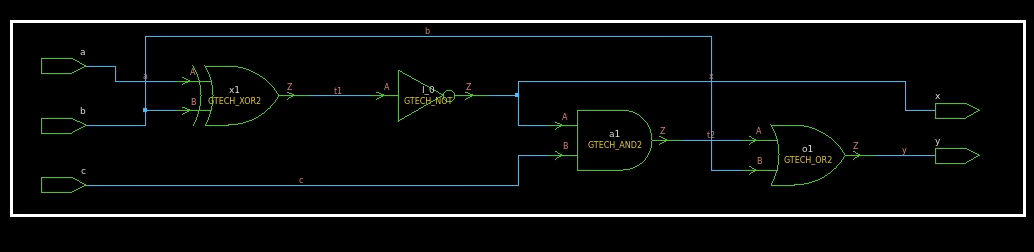
\includegraphics[width=0.8\textwidth]{question2a.png}
  \end{center}

  \item Critical path and delay:\par
  The critical path from primary input to output is
  \[
    a \rightarrow \text{xor} \rightarrow \text{not} \rightarrow \text{and} \rightarrow \text{or} \rightarrow y
  \]
  Total delay: 9 unit delays.
\end{enumerate}

\section*{Problem 4}
\noindent%
\begin{minipage}[t]{0.48\linewidth}
  \begin{enumerate}[label=(\alph*)]
    \item Part-logic and whole-logic modules:

    \textbf{Part-logic module}

    \begin{lstlisting}[style=verilog]
module part-logic(x,y,a,b,c);
  input a,b,c;
  output y,x;
  wire t1;
  not n1(t1,b);
  and a1(x,a,t1);
  or  o1(y,x,c);
endmodule
    \end{lstlisting}

    \textbf{Whole-logic module}

    \begin{lstlisting}[style=verilog]
module whole-logic(x,y,a,c,b);
  input [2:0] a;
  input [2:0] b;
  input c;
  output [2:0] x;
  output y;
  wire c1,c2;
  part-logic p11(x[0],c1,a[0],b[0],c);
  part-logic p12(x[1],c2,a[1],b[1],c1);
  part-logic p13(x[2],c,a[2],b[2],c2);
endmodule
    \end{lstlisting}
  \end{enumerate}
\end{minipage}%
\hfill%
\begin{minipage}[t]{0.48\linewidth}
  \begin{enumerate}[label=(\alph*),start=2]
    \item Using continuous assignment statement:

    \begin{lstlisting}[style=verilog]
module part-logic(x,y,a,b,c);
  input a,b,c;
  output x,y;
  assign x = a & (~b);
  assign y = x | c;
endmodule
    \end{lstlisting}
  \end{enumerate}
\end{minipage}

\section*{Problem 5}
SECDED (13,8) Hamming: positions 1,2,4,8 are parity; positions 3,5,6,7,9,10,11,12 are data; position 13 is overall parity $p_0$.

\noindent\textbf{Encoder}
\begin{lstlisting}[style=verilog]
// data[7:0] -> code[12:0] (1-based positions noted)
module hamming13_enc(input  [7:0] data, output [12:0] code);
  wire p1 = data[0]^data[1]^data[3]^data[4]^data[6];        // pos1
  wire p2 = data[0]^data[2]^data[3]^data[5]^data[6];        // pos2
  wire p4 = data[1]^data[2]^data[3]^data[7];                // pos4
  wire p8 = data[4]^data[5]^data[6]^data[7];                // pos8
  assign code = {
    ^{data,p1,p2,p4,p8},    // pos13 = p0 (overall even parity)
    data[7], data[6], data[5], data[4],                      // pos12..9
    p8,                                                       // pos8
    data[3], data[2], data[1],                               // pos7..5
    data[0],                                                 // pos3
    p4,                                                      // pos4
    p2,                                                      // pos2
    p1                                                       // pos1 (LSB)
  };
endmodule
\end{lstlisting}


\newpage

\noindent\textbf{Decoder with single-error correction + double-error detect}
\begin{lstlisting}[style=verilog]
module hamming13_dec(
  input  [12:0] code_in,
  output [7:0]  data_out,
  output        err_single, err_double
);
  // unpack per position (1-based for clarity)
  wire p1 = code_in[0],  p2 = code_in[1],  d0 = code_in[2],  p4 = code_in[3];
  wire d1 = code_in[4],  d2 = code_in[5],  d3 = code_in[6],  p8 = code_in[7];
  wire d4 = code_in[8],  d5 = code_in[9],  d6 = code_in[10], d7 = code_in[11];
  wire p0 = code_in[12];

  wire s1 = p1 ^ d0 ^ d1 ^ d3 ^ d4 ^ d6;
  wire s2 = p2 ^ d0 ^ d2 ^ d3 ^ d5 ^ d6;
  wire s4 = p4 ^ d1 ^ d2 ^ d3 ^ d7;
  wire s8 = p8 ^ d4 ^ d5 ^ d6 ^ d7;
  wire [3:0] syndrome = {s8,s4,s2,s1};       // 1..12
  wire parity_err = ^code_in;                // overall parity check (even)

  reg [12:0] corrected;
  always @* begin
    corrected = code_in;
    if (syndrome != 0 && parity_err)          // single-bit error in 1..12
      corrected[syndrome-1] = ~code_in[syndrome-1];
    else if (syndrome == 0 && parity_err)     // error only in p0
      corrected[12] = ~code_in[12];
  end

  assign err_single = (syndrome != 0 && parity_err) || (syndrome == 0 && parity_err);
  assign err_double = (syndrome != 0 && !parity_err);  // detected, not corrected

  assign data_out = {corrected[11],corrected[10],corrected[9],corrected[8],
                     corrected[6],corrected[5],corrected[4],corrected[2]};
endmodule
\end{lstlisting}

\end{document}
